\documentclass[border=6pt]{standalone}
\usepackage{tikz}
\usetikzlibrary{arrows.meta,positioning,shapes.geometric}
\begin{document}
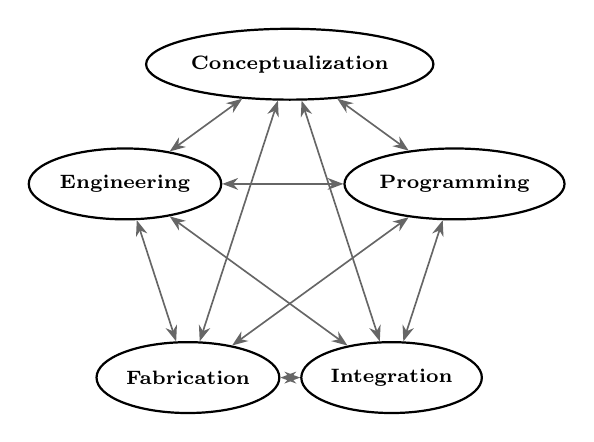
\begin{tikzpicture}[
    node/.style={ellipse, draw=black, thick, minimum height=0.9cm, minimum width=1.1cm, font=\scriptsize\bfseries, inner sep=1pt},
    connection/.style={Stealth-Stealth, black!60, semithick}
]
    \node[node] (concept) at (90:2.2cm) {Conceptualization};
    \node[node] (elec) at (162:2.2cm) {Engineering};
    \node[node] (prog) at (234:2.2cm) {Fabrication};
    \node[node] (enc) at (306:2.2cm) {Integration};
    \node[node] (int) at (18:2.2cm) {Programming};

    \draw[connection] (concept) -- (elec);
    \draw[connection] (concept) -- (prog);
    \draw[connection] (concept) -- (enc);
    \draw[connection] (concept) -- (int);
    \draw[connection] (elec) -- (prog);
    \draw[connection] (elec) -- (enc);
    \draw[connection] (elec) -- (int);
    \draw[connection] (prog) -- (enc);
    \draw[connection] (prog) -- (int);
    \draw[connection] (enc) -- (int);
\end{tikzpicture}
\end{document}
